\section{Summary Statistics and Covariates}\label{app:sumstats}

In this section we display summary statistics about the CPUMA-level datasets. The first two tables pertain to treatment assignment classifications. Table~\ref{tab:txassign} lists the states that are assigned to each group: the first two columns include the treatment states and control states in our primary analysis. The third column lists the treatment states for our sensitivity analysis that excludes ``early expansion'' states. The final column indicates states that were always excluded from the analysis. Table~\ref{tab:cpumasperstate} displays the total number of CPUMAs per state, as well as a column reiterating the state's treatment assignment and whether it was an early expansion state.

The subsequent tables and figure display summary information about the expansion state data and the homogeneous and heterogeneous covariate adjustments detailed in Appendix~\ref{app:adjustmentdetails}. 

Table~\ref{tab:summarytab1} displays univariate summary statistics for the treated CPUMAs. Specifically, the table displays mean, interquartile range, and the range (as defined by the maximum value minus the minimum value) for the unadjusted dataset, the heterogeneous adjustment, and the homogeneous adjustment. We see that the covariate adjustments generally reduce the variability relative to the unadjusted data. 

Table~\ref{tab:extreme1} displays the frequency that the adjusted covariates fell outside of the support of the unadjusted dataset on our primary dataset. The frequency is comparable for either adjustment and the counts are low, supporting the use of the linear model outlined in \eqref{eqn:regcal}. We also calculate these adjustments excluding early expansion states, and recalculate these adjustments excluding each state one at a time to calculate our variance estimates, yielding different results with respect to the quality of the resulting adjustments. These results are available on request.

Table~\ref{tab:timetrends} displays the trends in the outcome over time by treatment group. We use these estimates to compute the difference-in-differences estimator of the ETT in footnote \ref{footnote_did}. 

Figure~\ref{fig:corrmatrix} displays the Pearson's correlation coefficients for the bivariate relationships between the covariates on the unadjusted dataset (including both treated and untreated units). These point estimates may be biased due to the measurement error in the covariates. Nevertheless, this matrix is useful for at least two reasons: first, assuming the correlations among the treated and untreated units are similar, the more heavily correlated the data the easier it should be to attain covariate balance (see, e.g., \citet{d2021overlap}). This matrix gives a general sense of how correlated the data are, even if the estimates are biased. Second, these correlations can suggest potential confounders by revealing which variables are most heavily associated with treatment assignment and the pre-treatment outcomes. For example, the plot shows a strong association between Republican governance and treatment assignment, and a smaller association between these variables with pre-treatment outcomes. The plot also illustrates strong associations between the pre-treatment uninsurance rates, though they are more weakly associated with treatment assignment. 

\begin{table}[h!]\caption{Treatment assignment classification}\label{tab:txassign}
\centering
%\hline 
\begin{tabularx}{\textwidth}{XXXX} \\ 
Treated states & Control states & Early expansion states & Always excluded \\ 
\hline
AR, AZ, CA, CO, CT, HI, IA, IL, KY, MD, MI$^\textrm{a}$, MN, ND, NJ, NM, NV, OH, OR, RI, WA, WV & AK, AL, FL, GA, ID, IN, KS, LA, ME, MO, MS, MT, NC, NE, OK, PA, SC, SD, TN, TX, UT, VA, WI, WY & CA, CT, MN, NJ, WA & DE$^\textrm{c}$, MA$^\textrm{c}$, NH$^\textrm{b}$, NY$^\textrm{c}$, VT$^\textrm{c}$, DC$^\textrm{c}$\\ 
\hline 
\end{tabularx} {
     \vspace{1ex} }
     {\par \raggedright $^\textrm{a}$ Expanded April 2014 \par 
     \raggedright $^\textrm{b}$ Expanded September 2014; included for covariate adjustment estimates but not as a possible weight donor for treatment effect estimates \par 
    \raggedright $^\textrm{c}$ Comparable coverage policies prior to 2014 
    \par}
\end{table}

\begin{table}[ht]
\centering
\caption{Number of CPUMAs per state}\label{tab:cpumasperstate}
\begin{tabular}{lllrl}
  \hline
State Full & State & Treatment & Number CPUMAs & Early Expansion \\ 
  \hline
Delaware & DE & Excluded &   4 & No \\ 
  Massachusetts & MA & Excluded &  15 & No \\ 
    New Hampshire & NH & Excluded $^\textrm{a}$ &   4 & No \\ 
  New York & NY & Excluded & 123 & No \\ 
  Vermont & VT & Excluded &   4 & No \\ 
  Arizona & AZ & Expansion &  11 & No \\ 
  Arkansas & AR & Expansion &  15 & No \\ 
  Colorado & CO & Expansion &  15 & No \\ 
  Hawaii & HI & Expansion &   8 & No \\ 
  Illinois & IL & Expansion &  47 & No \\ 
  Iowa & IA & Expansion &   7 & No \\ 
  Kentucky & KY & Expansion &  23 & No \\ 
  Maryland & MD & Expansion &  36 & No \\ 
  Michigan & MI & Expansion &  44 & No \\ 
  Nevada & NV & Expansion &   7 & No \\ 
  New Mexico & NM & Expansion &   6 & No \\ 
  North Dakota & ND & Expansion &   2 & No \\ 
  Ohio & OH & Expansion &  44 & No \\ 
  Oregon & OR & Expansion &  17 & No \\ 
  Rhode Island & RI & Expansion &   6 & No \\ 
  West Virginia & WV & Expansion &   4 & No \\ 
  California & CA & Expansion & 110 & Yes \\ 
  Connecticut & CT & Expansion &  22 & Yes \\ 
  Minnesota & MN & Expansion &  27 & Yes \\ 
  New Jersey & NJ & Expansion &  38 & Yes \\ 
  Washington & WA & Expansion &  22 & Yes \\ 
  Alabama & AL & Non-expansion &  18 & No \\ 
  Alaska & AK & Non-expansion &   4 & No \\ 
  Florida & FL & Non-expansion &  59 & No \\ 
  Georgia & GA & Non-expansion &  20 & No \\ 
  Idaho & ID & Non-expansion &   1 & No \\ 
  Indiana & IN & Non-expansion &  24 & No \\ 
  Kansas & KS & Non-expansion &   9 & No \\ 
  Louisiana & LA & Non-expansion &  15 & No \\ 
  Maine & ME & Non-expansion &   5 & No \\ 
  Mississippi & MS & Non-expansion &   7 & No \\ 
  Missouri & MO & Non-expansion &  16 & No \\ 
  Montana & MT & Non-expansion &   1 & No \\ 
  Nebraska & NE & Non-expansion &  11 & No \\ 
  North Carolina & NC & Non-expansion &  27 & No \\ 
  Oklahoma & OK & Non-expansion &   8 & No \\ 
  Pennsylvania & PA & Non-expansion &  55 & No \\ 
  South Carolina & SC & Non-expansion &  10 & No \\ 
  South Dakota & SD & Non-expansion &   1 & No \\ 
  Tennessee & TN & Non-expansion &  28 & No \\ 
  Texas & TX & Non-expansion &  49 & No \\ 
  Utah & UT & Non-expansion &   8 & No \\ 
  Virginia & VA & Non-expansion &  15 & No \\ 
  Wisconsin & WI & Non-expansion &  21 & No \\ 
  Wyoming & WY & Non-expansion &   2 & No \\ 
   \hline
\end{tabular}
     \vspace{1ex}
     \newline
     {\raggedright $^\textrm{a}$ Included for covariate adjustment estimates but not as a possible weight donor for treatment effect estimates \par }
\end{table}

\begin{table}[h!]
\centering
\caption{Univariate summary statistics on adjusted data, primary dataset \\ (Mean, IQR, Range)}\label{tab:summarytab1}
\begin{tabular}{rllll}
  \hline
Variable & Unadjusted & Heterogeneous & Homogeneous \\ 
  \hline
  Age: 19-29 Pct & (24.5, 6, 30.9) & (24.5, 5.9, 29) & (24.5, 5.9, 29) \\ 
  Age: 30-39 Pct & (20.9, 3.4, 20.9) & (20.9, 3.1, 19.1) & (20.9, 3.1, 19.4) \\ 
  Age: 40-49 Pct & (22.2, 2.5, 15.4) & (22.2, 2.3, 13.7) & (22.2, 2.2, 13.7) \\ 
  Avg Adult to Household Ratio & (151, 27.2, 174.3) & (151, 27.2, 173.8) & (151, 27.2, 173.3) \\ 
  Avg Pop Growth & (100.3, 1.9, 13.7) & (100.3, 1.2, 6.2) & (100.3, 1.2, 6.5) \\ 
  Children: Missing Pct & (10.5, 6.6, 41) & (10.5, 6.5, 40.8) & (10.5, 6.5, 40.5) \\ 
  Children: One Pct & (11.1, 3.1, 14.3) & (11.1, 2.8, 12.3) & (11.1, 2.8, 12.5) \\ 
  Children: Three or More Pct & (5.2, 2, 14.1) & (5.2, 1.7, 13.5) & (5.2, 1.7, 13.3) \\ 
  Children: Two Pct & (9.7, 3.5, 15) & (9.7, 3.3, 13.5) & (9.7, 3.2, 13.6) \\ 
  Citizenship Pct & (90, 11.9, 57.1) & (90, 11.8, 55.4) & (90, 11.7, 55.7) \\ 
  Disability Pct & (10.5, 5.3, 28.6) & (10.4, 5.3, 26.7) & (10.5, 5.4, 27.2) \\ 
  Educ: HS Degree Pct & (26.3, 10.7, 43.2) & (26.3, 10.6, 41.8) & (26.3, 10.6, 42) \\ 
  Educ: Less than HS Pct & (11.4, 7.7, 45.3) & (11.4, 7.5, 45) & (11.4, 7.4, 44.6) \\ 
  Educ: Some College Pct & (33.5, 7.9, 34.2) & (33.5, 7.5, 32.9) & (33.5, 7.4, 33) \\ 
  Female Pct & (50.1, 1.6, 15.4) & (50.1, 1.4, 14.2) & (50.1, 1.5, 14.2) \\ 
  Foreign Born Pct & (18.1, 22.4, 76) & (18.1, 22.2, 75.2) & (18.1, 22.2, 75.4) \\ 
  Hispanic Pct & (15.9, 17.7, 97.2) & (15.9, 17.7, 97) & (15.9, 17.7, 97) \\ 
  Inc Pov: $<$ 138 Pct & (20, 11.9, 45.6) & (20, 11.8, 44.8) & (20, 11.8, 43.9) \\ 
  Inc Pov: 139-299 Pct & (24.9, 8.4, 34.2) & (24.9, 7.9, 34.2) & (24.9, 7.8, 34.1) \\ 
  Inc Pov: 300-499 Pct & (23.6, 5.5, 23) & (23.6, 4.9, 22.2) & (23.6, 4.9, 22.2) \\ 
  Inc Pov: 500 + Pct & (29.3, 18.5, 69.1) & (29.3, 18.5, 68.1) & (29.3, 18.5, 68) \\ 
  Married Pct & (50.7, 9.4, 45.1) & (50.7, 9, 44.1) & (50.7, 9.1, 44.2) \\ 
  Race: White Pct & (73.8, 25.4, 91.9) & (73.8, 25.5, 91.7) & (73.8, 25.5, 91.8) \\ 
  Republican Governor 2013 $^\textrm{a}$& (31.1, 100, 100) & (31.1, 100, 100) & (31.1, 100, 100) \\ 
  Republican Lower Leg Control 2013 $^\textrm{a}$ & (24.1, 0, 100) & (24.1, 0, 100) & (24.1, 0, 100) \\ 
  Republican Total Control 2013 $^\textrm{a}$ & (19.8, 0, 100) & (19.8, 0, 100) & (19.8, 0, 100) \\ 
Student Pct & (11.7, 3.4, 29.5) & (11.7, 3.5, 28.1) & (11.7, 3.5, 28) \\ 
  Unemployed Pct 2011 & (10.2, 4.6, 25.5) & (10.2, 3.9, 23.8) & (10.2, 3.9, 22.5) \\ 
  Unemployed Pct 2012 & (9.4, 4.5, 28.3) & (9.4, 4.3, 23.6) & (9.4, 4.3, 23.5) \\ 
  Unemployed Pct 2013 & (8.4, 3.6, 23.4) & (8.4, 3.5, 20.1) & (8.4, 3.5, 20.5) \\ 
  Uninsured Pct 2011 & (19.6, 11.2, 59) & (19.7, 10.9, 51.8) & (19.6, 10.9, 52.5) \\ 
  Uninsured Pct 2012 & (19.4, 9.9, 50.6) & (19.4, 10.1, 49.7) & (19.4, 10.3, 50.2) \\ 
  Uninsured Pct 2013 & (19, 11.2, 49.9) & (19, 10.3, 48.2) & (19, 10.5, 48.7) \\ 
  Urban Pct $^\textrm{b}$ & (82.9, 31.3, 91.3) & (82.9, 31.3, 91.3) & (82.9, 31.3, 91.3) \\ 
   \hline
\end{tabular}
     \vspace{1ex}
     
     {\raggedright $^\textrm{a}$ Derived from data obtained from National Conference of State Legislatures \par
     $^\textrm{b}$ Derived from 2010 Census \par
     }
\end{table}

\begin{table}[h!]
\centering
    \caption{Frequency of covariate adjustments falling outside the support of the unadjusted data \newline (primary dataset)}
    \label{tab:extreme1}
\begin{tabular}{lll}
  \hline
Variables & Heterogeneous & Homogeneous \\ 
  \hline
Age: 19-29 Pct & 0 & 0 \\ 
  Age: 30-39 Pct & 0 & 0 \\ 
  Age: 40-49 Pct & 0 & 0 \\ 
  Avg Adult to Household Ratio & 0 & 0 \\ 
  Citizenship Pct & 1 & 0 \\ 
  Disability Pct & 2 & 2 \\ 
  Educ: HS Degree Pct & 0 & 0 \\ 
  Educ: Less than HS Pct & 1 & 1 \\ 
  Educ: Some College Pct & 0 & 0 \\ 
  Female Pct & 0 & 0 \\ 
  Foreign Born Pct & 1 & 1 \\ 
  Uninsured Pct 2011 & 0 & 0 \\ 
  Uninsured Pct 2012 & 1 & 1 \\ 
  Uninsured Pct 2013 & 0 & 1 \\ 
  Hispanic Pct & 0 & 0 \\ 
  Inc Pov: $<$ 138 Pct & 1 & 1 \\ 
  Inc Pov: 139-299 Pct & 1 & 1 \\ 
  Inc Pov: 300-499 Pct & 0 & 0 \\ 
  Inc Pov: 500 + Pct & 0 & 0 \\ 
  Married Pct & 0 & 0 \\ 
  Children: Missing Pct & 1 & 1 \\ 
  Children: One Pct & 0 & 0 \\ 
  Avg Pop Growth & 0 & 0 \\ 
  Race: White Pct & 1 & 1 \\ 
  Student Pct & 0 & 0 \\ 
  Children: Three or More Pct & 2 & 1 \\ 
  Children: Two Pct & 1 & 1 \\ 
  Unemployed Pct 2011 & 0 & 0 \\ 
  Unemployed Pct 2012 & 0 & 0 \\ 
  Unemployed Pct 2013 & 0 & 0 \\ 
   \hline
\end{tabular}
\end{table}

\begin{table}[ht]
\centering
\caption{Mean non-elderly adult uninsurance rates, 2009-2014}\label{tab:timetrends}
\begin{tabular}{lrrrrrr}
  \hline
Treatment Group & 2009 & 2010 & 2011 & 2012 & 2013 & 2014 \\ 
  \hline
Non-expansion & 21.84 & 22.97 & 22.72 & 22.41 & 22.01 & 19.07 \\ 
  Expansion (primary dataset) & 19.52 & 20.20 & 19.63 & 19.42 & 19.01 & 14.02 \\ 
  Expansion (early excluded) & 19.40 & 20.08 & 19.21 & 19.01 & 18.55 & 13.64 \\ 
   \hline
\end{tabular}
\end{table}

\begin{figure}[h!]
\begin{center}
    \caption{Correlation matrix: full data, unadjusted covariates \newline (primary dataset)}
    \label{fig:corrmatrix}
    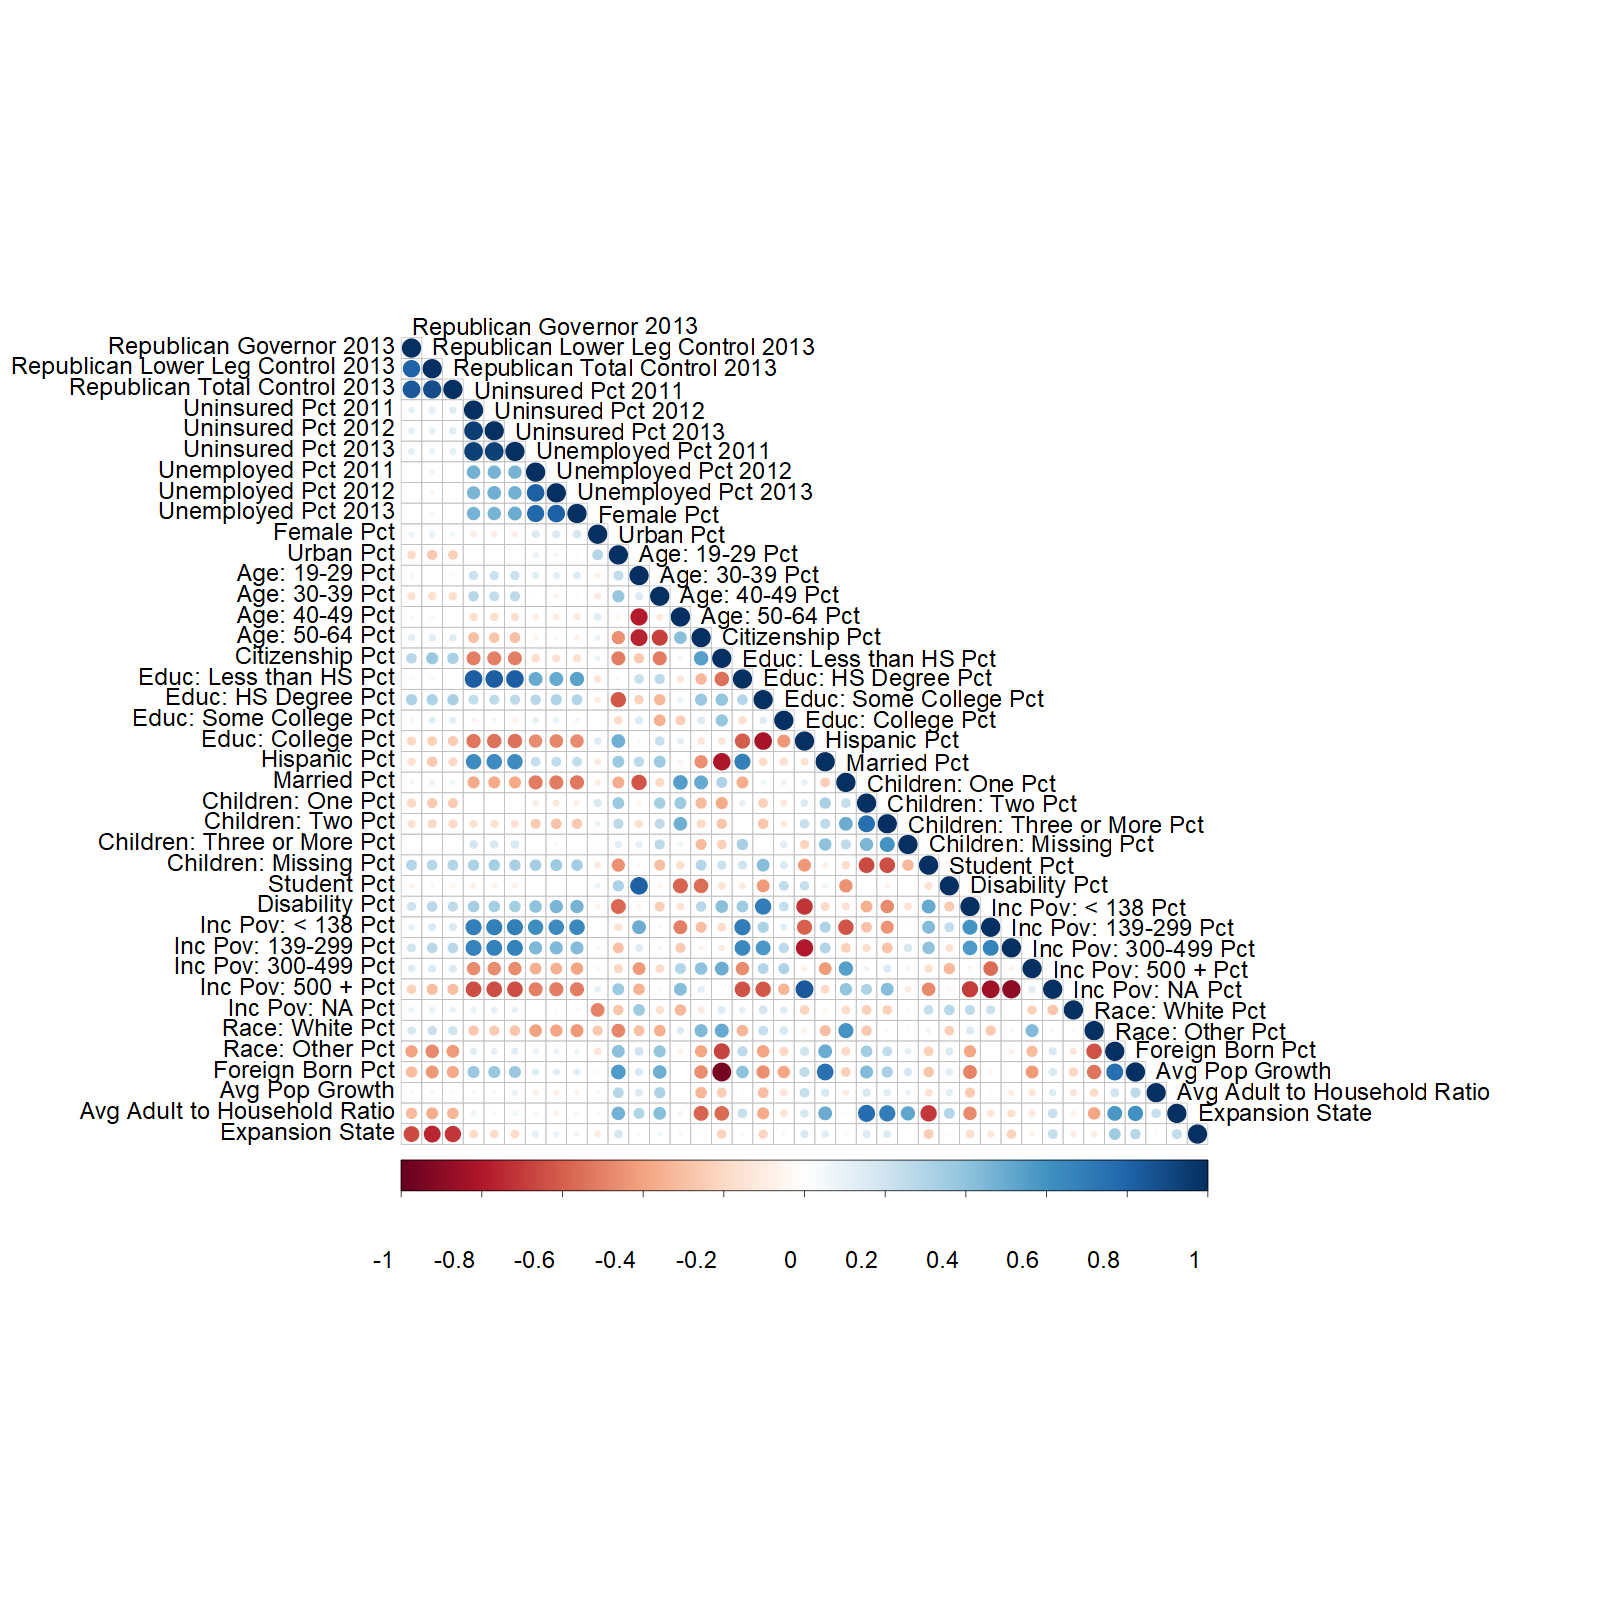
\includegraphics[scale=0.25]{01_Plots/correlation-plot-c1-sigma-zero.png}
\end{center}
\end{figure}

\clearpage